\newcommand{\labname}{HW3}
\documentclass[11pt]{article}
\usepackage[left=1in, right=1in, top=1in, bottom=1in]{geometry}
\usepackage{amsmath,amsfonts,amssymb}
\usepackage{graphicx}
\usepackage{fancyhdr}
\usepackage{tikz}
\usepackage{wrapfig}
\usepackage{pgfplots}
\usepackage{setspace}
\usepackage{float}
\usepackage{multirow}
\doublespacing
% TODO: CHANGE THESE
\newcommand{\myname}{Di Wang}
\newcommand{\myandrewid}{diw2}
\newcommand{\myrecitation}{B}

% LSTLISTINGS PACKAGE (for pseudocode) ======================================
\usepackage{listings}

\newdimen\zzsize
\zzsize=11pt
\newdimen\kwsize
\kwsize=11pt

\newcommand{\basicstyle}{\fontsize{\zzsize}{1.1\zzsize}\ttfamily}
\newcommand{\keywordstyle}{\fontsize{\kwsize}{1.1\kwsize}\normalfont\bf}
\newlength{\zzlstwidth}
\settowidth{\zzlstwidth}{{\basicstyle~}}
\newcommand{\lcm}{}

\lstset{
  xleftmargin=5.0ex,
  basewidth=\zzlstwidth,
  basicstyle=\basicstyle,
  captionpos=b,
  numbers=left, numberstyle=\small, numbersep=8pt,
  keywordstyle=\keywordstyle,
  keywords={signature,sig,structure,struct,function,fun,fn,case,of,type,datatype,let,val,fn,in,end,as,functor,alloc,if,then,else,while,with,and,start,do},
  commentstyle=\rmfamily\slshape,
  morecomment=[l]{\%},
  lineskip={1.5pt},
  columns=[l]fullflexible,
  keepspaces=true,
  mathescape=true,
  escapeinside={@}{@},
% NOTE: need TWO sets of braces around each definition below!
  literate={requires}{{$\lcm\text{\keywordstyle \% requires}$}}6
           {returns}{{$\lcm\text{\keywordstyle \% returns}$}}6
           {=}{{$\lcm=$}}2
           {(}{{$($}}2
           {)}{{$)$}}2
           {**}{{$\lcm\times$}}2
%           {||}{{$\lcm\Vert$}}2
           {|}{{$|$}}2
           {=>}{{$\lcm\boldsymbol\Rightarrow$}}2
           {->}{{$\lcm\rightarrow$}}2
           {'a}{{$\alpha$}}1
           {'b}{{$\beta$}}1
}
% END LSTLISTINGS PACKAGE ===================================================

% header
\pagestyle{fancy}
\fancyhf{}
\lhead{Parallel Go Solver}
%\chead{\myname{} (\myandrewid)}
\chead{Bo Gao, Di Wang}
%\rhead{Page \thepage{} of \pageref{mylastpagelabel}}
\rhead{December 2017}
\lfoot{}
\rfoot{\bf \thepage}
\cfoot{}
% document starts
\begin{document}
\linespread{1.5}
{\centering
{\huge \bfseries Final Project report \par}
\vspace{0.5cm}
{\Large Bo Gao(bgao), Di Wang(diw2) \par}}

\section*{Summary}
We implemented a parallel Go artificial intelligence (AI) program in CUDA on the GPU. Our implementation achieved perfect accuracy when used to solve life-and-death problems (tsumego) on the corners and edges. The interactive AI could win games against amateur players without dan grading, with a considerably fast speed. It also sometimes provided elegant moves that could be great examples for beginners.
\section*{Background}
Go is an abstract strategy zero-sum board game for two players, in which the aim is to surround more territory than the opponent. Our interactive application is an AI creating a computer program that plays the game with users. Because of its complexity and different patterns involved, the minimax search method used in chess alone may not work, as there can be in total $3^{19 \times 19} = 3^{361}$ different board compositions. Therefore a Go AI with the same sophistication level as a professional champion had always been an important research of study, as it was said to be able to model human thinking \cite{SN}.
\\
However, with the advent of AlphaGo in March 2016, and AlphaGo Zero in May 2017, more and more AIs become able to beat professional Go players. All of them use deep learning to train the neural network, both from human and computer playing \cite{NA}. This includes both pattern matching on partial boards, as well as pan-board calculations.\\
Because we lacked the knowledge of complex pattern matching, we decided to use only the idea of mini-max and Alpha Beta pruning, and to try to incorporate parallelism using CUDA. The minimax search here is definitely the most expensive part of the program, and it can benefit a lot from parallelism. Also, the good thing is there would be no dependencies between different paths as long as they do not write on the global board.\\
However, without ways to bring down the total number of moves to search for using the aforementioned pattern matching idea, we would try to come up with some heuristic that would allow us to judge the board state. In other words, we would examine the board state and give a score for Black. If it is Black's move it would want to maximize the minimum of all future scores after the next White's move, and vice versa for White. This is the minimax algorithm. In fact, after some trials and observations on the AI's moves, we finds out that the Monte-Carlo Tree Search algorithm may perform better on the moves. The MCTS algorithm basically generates some random moves afterwards, and returns the optimal first move with the highest average efficiency of territory surrounding. The only difference with Minimax Tree is that we use a find-max-average iteration instead of a find-max-min iteration after each potential-move-sequences returns its evaluation. \newline
In addition, our algorithm would also include Alpha-beta pruning which is an adversarial search algorithm used commonly for machine playing of two-player games. It is a search algorithm that seeks to decrease the number of nodes that are evaluated by the minimax algorithm in its search tree. It stops completely evaluating a move when at least one possibility has been found that proves the move to be worse than a previously examined move. Such moves need not be evaluated further. We would use this to bring down the total number of checks. \\
Various research has been done on the heuristic for board/move evaluation \cite{ME}. However, even for a rough approximation, considerable accuracy is only achieved by training in a convolutional neural network. The more layers, the higher the accuracy, but even so the maximum accuracy achieved is only $ \ 55.2\%$ \cite{ME}, which leaves room for improvement, but this is not an important topic in this project. We would adopt a similar heuristic, yet simpler. \\
\section*{Approach}
Our project included a User Interface (UI) in Java, and everything else in C$++$. We first spend time on building the Java interactive UI, which is a completely distinct program from the AI implemented using C++ and specifically CUDA. The interactive UI lets the player play Black, and then responds with a White move. The UI and underlying decision implementation are linked by Java Native Interface (JNI). \\
Then we began to implement the life-and-death problem solver. This is also a good starting point for the full game AI. Without loss of generality we made all the problems starting by White, with an attempt to kill the Black piece. Our algorithm would be the combination of minimax and Alpha-Beta discussed in \textbf{Background}. Here is an illustration of Alpha-Beta pruning:
\begin{figure}[H]
    \centering
    \includegraphics[width=0.5\textwidth]{Alpha_Beta.png}
    \caption{Alpha Beta Pruning \cite{AB}}
\end{figure}
Our algorithm for the life-and-death problems is a little different, as the end state would result in either the Black piece DEAD or ALIVE. Also, it is possible to infer from the exact shape of the Black piece whether it is alive or dead, even before all the possibilities are exhausted. This is essentially the same as pruning, as it eliminates possibilities that are about to result in Black alive from the perspective of White, or Black dead for Black. \\
Therefore our sequential algorithm would exhaust all the possible end states using Alpha-Beta pruning. The parallel algorithm, on the other hand, would parallel on the combined state of first $n$ moves, where $n$ is to be varied. Each life-and-death problem has a fixed finite number of crosses to be searched for, which we call $m$. For example, the following problem has $m = 5$. 
\begin{figure}[H]
    \centering
    \includegraphics[width=0.3\textwidth]{ld_pro_1.png}
    \caption{Example life and death problem with $m = 5$}
\end{figure}
For this problem, we are parallelizing on the first White move. Therefore the total number of threads would be 5 in this case. Each CUDA thread, in the kernel, would get a copy of the board state with the first two moves placed, and then use the aforementioned Alpha-Beta pruning algorithm to decide if this path has all subsequent paths resulting in DEAD or at least one resulting in ALIVE. Then the sequential algorithm on the host would use this to decide if White can kill the Black, and if so, under which move(s). \\
The results for the solver are accurate on $m \leq 8$ with considerable speed. This will be analyzed more in \textbf{Result}. \\
With this life-and-death problem solver handy, we were able to implement the full game AI. As introduced in \textbf{Background}, the number of possible Go board states greatly exceeds that of other board games, making it impossible to do a brute force search on all the possibilities. The approach we took was, again, parallelize on most of all possible board states after $n$ moves, where $n$ can be varied. We were able to use some Go intuition to eliminate many of the blatantly bad cases, for example when jumping far from the last opponent's move, or placing in a dangerous cross soon to be captured (examples below).
\begin{figure}[H]
    \centering
    \includegraphics[width=0.3\textwidth]{bad_1.png}
    \caption{Example bad move by White, as Black can capture it within one move.}
\end{figure}
\begin{figure}[H]
    \centering
    \includegraphics[width=0.3\textwidth]{bad_2.png}
    \caption{Example bad move by White, as it wanders off the current battlefield.}
\end{figure}
The moves like above would not be included in our CUDA search. In other words, we would only look at moves that are closer to the last opponent's move, and that make some Go-intuitive sense.  Without this clever search, we would have to say with $n = 2$, with $361^2$ threads. With the precheck implemented, we are able to make $n$ as great as 6. \\
The rest of the parallel algorithm works similarly to the one used in the parallel life-and-death problem solver. However, since we do not reach the end game at the end of the $n$th step, instead of deciding DEAD or ALIVE, we would use a heuristic similar to the one referred to in \textbf{Background} to determine the current board state. Our heuristic works like a model of magnetic field of different magnets: each stone can be seen as a magnetic, that exerts force on points close to it. The closer the point, the greater the influence. Black influence and White influence cancel each other. Also, the edges and corners of the board act as ``mirrors'' so the magnetic field can bounce back. This is to represent the fact that stones on corners and edges have better control over the territory, than stones in the middle. \\
In summary, there are not much dependencies in the program except for the original, current board state to search from. Therefore, parallelism would be very amenable and applicable for the searches. Our model is similar to data parallel, as each part of the input array would be mapped to an output array without communication. It should also have a good temporal and spatial locality.
\section*{Trials and Iterations}
Our design and approach described above went through a series of trials and revises. Given the fact that Go is a board game where new stones were being added, and previous multiple stones might be captured at once, the checking algorithm needed careful recursion which is sometimes not able to be parallelized. Here are the problems that we encountered which changed our approach:
\begin{enumerate}
\item CUDA not fit for OOP: We first designed the game semantics in an object-oriented programing (OOP) style. However, we soon realized that in CUDA, there is no way for device functions to call host functions. We first tried to get around that by converting everything to device, but this is not only confusing, hard to implement, but also slow in practice. Therefore we finally changed the idea and made it more adaptive by C++.
\item Host pointers not accessible to device: Similar to above, the device cannot access host struct pointers. Therefore we modified the structure again so that we were passing structs directly instead of their pointers. 
\item Limitation on size of stack in CUDA: it turned out that our kernel implementation, which would call many device functions interchangeably, would  make the stack exceed the default size of 1024. Therefore we had to increase that as we went along. 
\item Limitation on the number of device functions called: Our original approach for life-and-death problems had a host function invoke the kernel many times, but the results were mostly inaccurate. It turned out that in our implementation the kernel could only be called 5 times, and would silently die after that. Therefore we modified the division of work so that the host function would initialize the array with indicator bits telling which task each thread should perform. This is similar to the style in Assignment 2 Rendering.
\item Limitation on the GPU memory: Allocating a local memory with very huge size inside the GPU is forbidden. So that's why when we are doing the full-board AI with size 19, we are not able to create so many local copies of the board, while we are just considering the potential moves near the previous move by the other player. 
\end{enumerate}
To sum up, the kernel should only be used to calculate something or do some uniform operation, but not as a recursive routine. In order to avoid the above problems, we must delegate some tasks to the sequential part of the implementation.\\


\section*{Result}
%The distribution of work is $50\% - 50\%$.
We would analyze the results in two aspects: the running time performance and speedup in parallel life-and-death problem solver and full game AI, and the sophistication of the actual moves returned by the full game AI.\\
Here is the average performance comparison for the running times for the full game AI, with $n = 1$, on an actual board size of $19 \times 19$, for the first five steps. We compared the performance of the baseline single-threaded CPU code with the parallel CUDA code. The results were generated with the help of the code $\mathsf{cycleTimer.h}$ provided by the course.
\begin{table}[H]
\centering
\caption{Full game AI serialized vs. parallel}
\label{label1}
\begin{tabular}{|l|l|l|l|l|l|}
\hline
Steps & \begin{tabular}[c]{@{}l@{}}Time of serialized\\ algorithm on CPU\\ in milliseconds\end{tabular} & \begin{tabular}[c]{@{}l@{}}Time of parallel\\ algorithm on GPU\\ in milliseconds\end{tabular} & \begin{tabular}[c]{@{}l@{}}Time of Cuda \\ Kernel in \\ milliseconds\end{tabular} & \begin{tabular}[c]{@{}l@{}}Speedup in\\ terms of \\ running time\end{tabular} & \begin{tabular}[c]{@{}l@{}}Speedup in \\ terms of\\ kernel running time\end{tabular} \\ \hline
1     & 14.1435                                                                                         & 3.7785                                                                                        & 0.0227                                                                            & 3.74315                                                                       & 623.061674                                                                           \\ \hline
2     & 18.8677                                                                                         & 4.0783                                                                                        & 0.0190                                                                            & 4.62636                                                                       & 993.036842                                                                           \\ \hline
3     & 23.9899                                                                                         & 3.8899                                                                                        & 0.0183                                                                            & 6.16723                                                                       & 1310.9235                                                                            \\ \hline
4     & 26.4919                                                                                         & 3.8477                                                                                        & 0.0180                                                                            & 6.88512                                                                       & 1471.7722                                                                            \\ \hline
5     & 32.0519                                                                                         & 3.8028                                                                                        & 0.0287                                                                            & 8.42850                                                                       & 1116.79094                                                                           \\ \hline
\end{tabular}
\end{table}
%%%%%%
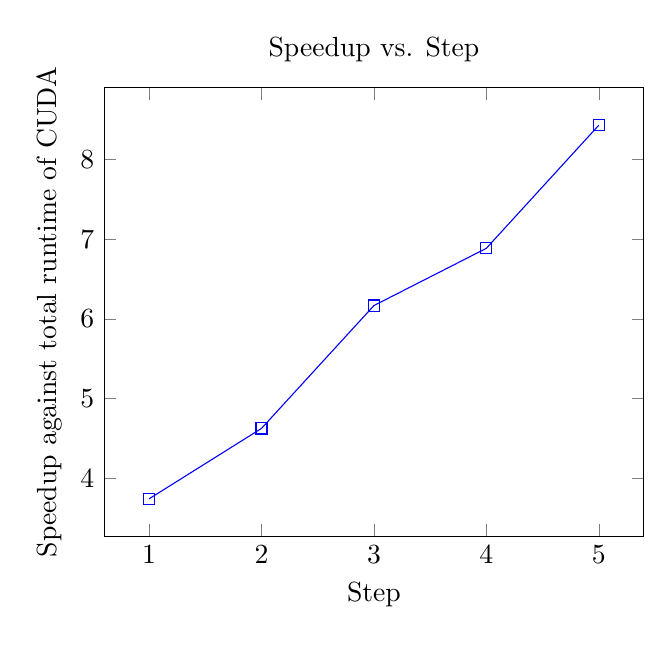
\begin{tikzpicture}
\begin{axis} [
  title={Speedup vs. Step},
  xlabel={Step},
  ylabel={Speedup against total runtime of CUDA},
  grid style=dashed,
]
\addplot[
  color=blue,
  mark=square,
  ]
  plot coordinates {
     (1, 3.74315)(2, 4.62636)(3, 6.16723)(4, 6.88512)(5, 8.42850)
  };
  %\addlegendentry{easy\_1024}
\end{axis}
\end{tikzpicture}
%%%
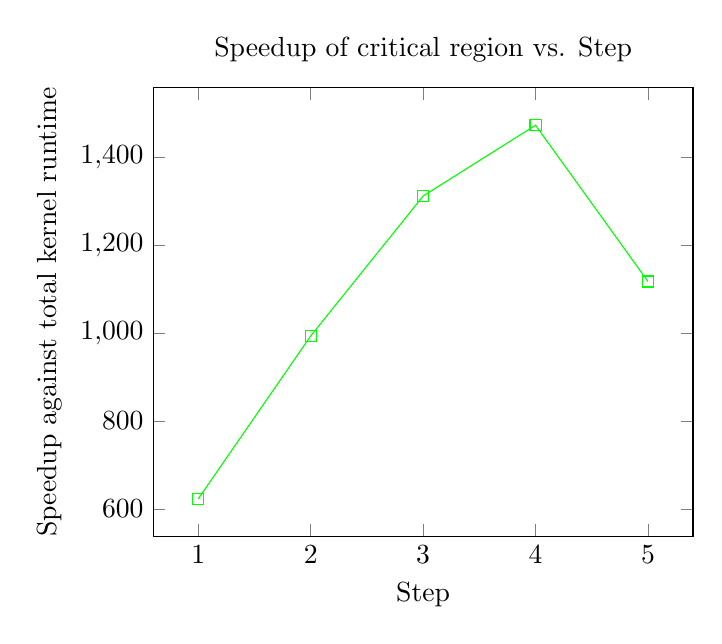
\begin{tikzpicture}
\begin{axis} [
  title={Speedup of critical region vs. Step},
  xlabel={Step},
  ylabel={Speedup against total kernel runtime},
  grid style=dashed,
]
\addplot[
  color=green,
  mark=square,
  ]
  plot coordinates {
     (1, 623.0616)(2, 993.0368)(3, 1310.9235)(4, 1471.7722)(5, 1116.79094)
  };
  %\addlegendentry{easy\_1024}
\end{axis}
\end{tikzpicture}
First of all, the reason that the sequential algorithm actually increases in runtime is because it needs the previously placed stones to calculate the potential board state of each proceeding path. This is not easily avoidable for the sequential algorithm, as it can only contain one copy of the board state at each timestamp (otherwise memory limit would be exceeded if each path has one copy). This is not the case for the CUDA parallel algorithm, because we have allocated enough memory and initialized the states for each possible path beforehand, which is the main difference between the columns \textit{Time of Cuda Kernel vs. Time of parallel algorithm}. \\
It turned out that the actual kernel computation was kept to a minimum, to our expectation as described in \textbf{Trials and Iterations}. Most of the expensive functions, such as \textit{stone\_add}, \textit{get\_state}, are no longer in the kernel, so the kernel only calls \textit{get\_terr}, which is the heuristic function, and returns it immediately. \\
\\
Next we repeat the experiment result above by changing the parameters. There  are two dimensions of variables to change: the board size $b$ ($b = 9$ means that the board is of size $9 \times 9$), and the depth of search defined in \textbf{Background}, $n$. Note that the above statistics are with $b = 19, n = 1$. Also, we are no longer calculating the kernel running time, as that is always very small and not a good parameter in the calculation of the speedup. 
\begin{table}[H]
\centering
\caption{Full game AI serialized vs. parallel cont.}
\label{my-label}
\begin{tabular}{|l|l|l|l|l|l|l|l|l|l|}
\hline
\multirow{2}{*}{Step} & \multicolumn{3}{l|}{Serialized runtime (ms)}                                                                                                                                        & \multicolumn{3}{l|}{Parallel runtime (ms)}                                                                                                                                          & \multicolumn{3}{c|}{Speedup}                                                                                                                                                        \\ \cline{2-10} 
                      & \begin{tabular}[c]{@{}l@{}}b = 9\\ n = 1\end{tabular} & \begin{tabular}[c]{@{}l@{}}b = 9\\ n = 2\end{tabular} & \begin{tabular}[c]{@{}l@{}}b = 19\\ n = 2\end{tabular} & \begin{tabular}[c]{@{}l@{}}b = 9\\ n = 1\end{tabular} & \begin{tabular}[c]{@{}l@{}}b = 9\\ n = 2\end{tabular} & \begin{tabular}[c]{@{}l@{}}b = 19\\ n = 2\end{tabular} & \begin{tabular}[c]{@{}l@{}}b = 9\\ n = 1\end{tabular} & \begin{tabular}[c]{@{}l@{}}b = 9\\ n = 2\end{tabular} & \begin{tabular}[c]{@{}l@{}}b = 19\\ n = 2\end{tabular} \\ \hline
1                     & 0.8601                                                    & 54.9245                                                   & 68.5128                                                     & 2.1970                                                    & 26.4787                                                   & 23.2450                                                     & 0.3914                                                    & 2.074                                                     & 2.947                                                       \\ \hline
2                     & 1.0967                                                    & 76.8910                                                   & 95.6443                                                     & 2.1112                                                    & 27.5114                                                   & 23.3673                                                     & 0.5195                                                    & 2.795                                                     & 4.093                                                       \\ \hline
3                     & 1.5444                                                    & 97.6486                                                   & 119.3768                                                    & 2.2408                                                    & 27.7287                                                   & 23.3265                                                     & 0.6892                                                    & 3.522                                                     & 5.118                                                       \\ \hline
4                     & 2.0792                                                    & 123.890                                                   & 147.3680                                                    & 2.1727                                                    & 27.6843                                                   & 23.7210                                                     & 0.9569                                                    & 4.475                                                     & 6.212                                                       \\ \hline
5                     & 2.3825                                                    & 143.503                                                   & 178.5760                                                    & 2.2378                                                    & 27.8785                                                   & 23.2771                                                     & 1.0646                                                    & 5.147                                                     & 7.671                                                       \\ \hline
\end{tabular}
\end{table} 
The general trend within each $b$ and $n$ is the same as the case in $b = 19$ and $n = 1$. We can also compare the results across the $b$'s and $n$'s. \\
Note that the trend on larger $b$ and $n$, the speedup increases. This is because if the problem size increases, the benefit of parallelism overweighs the overhead. Especially in the case of small problem size with $b = 9$ and $n = 1$, the overhead is so significant that the parallel algorithm runs slower than the serialized one for the first several steps. This confirms our expectation before the implementation. \\
\\
Next we do the same analysis on the performance of the life-and-death problem solver. We vary the number of available search points $m$ defined in \textbf{Background}.
\begin{table}[H]
\centering
\caption{Speedup of life-and-death problem solver}
\label{my-label}
\begin{tabular}{|l|l|l|l|l|l|l|l|}
\hline
\multirow{2}{*}{Iteration} & \multicolumn{3}{l|}{\begin{tabular}[c]{@{}l@{}}Average time of parallel algorithm \\  (ms)\end{tabular}} & \multicolumn{3}{l|}{\begin{tabular}[c]{@{}l@{}}Average time of serialized algorithm\\ (ms)\end{tabular}} & \multicolumn{1}{c|}{\begin{tabular}[c]{@{}c@{}}Average\\ Speedup\end{tabular}} \\ \cline{2-8} 
                           & m = 5                             & m = 4                             & m =3                             & m = 5                             & m = 4                             & m = 3                            & m = 3,4,5                                                                      \\ \hline
1                          & 2933.4                            & 770.04                            & 81.87                            & 11.59                             & 2.06                              & 1.30                             & 0.00395                                                                        \\ \hline
2                          & 2700.7                            & 789.72                            & 72.48                            & 11.37                             & 2.02                              & 1.30                             & 0.00258                                                                        \\ \hline
3                          & 2866.9                            & 807.96                            & 83.40                            & 11.38                             & 2.04                              & 1.24                             & 0.01619                                                                        \\ \hline
Avg                        & 2833.7                            & 789.24                            & 79.05                            & 11.45                             & 2.04                              & 1.28                             & 0.00757                                                                        \\ \hline
\end{tabular}
\end{table}
Much to our surprise, the parallel algorithm is much worse than the sequential algorithm. We conjecture that the overhead of the CUDA threads greatly outweighs any improvement by parallelism, since the parallel function only parallelizes the first several steps, which would not result in as big a speedup as in the case of the Go AI, as the search points is greatly reduced.\\
Therefore, increasing $m$ would definitely improve the speedup, which is also a trend we see from $m = 3$ to $m = 5$. However, after $m = 7$ the running time increases drastically, because the number of recursions that we are doing is increasing exponentially. Therefore we did not test on larger $m$'s. But for smaller problems parallelization might not be a good idea.\\
To sum up, the speedup for both full game AI and life-and-death problem solver did not meet our expectation. One of the most important reasons is a lack of parallelism. Our algorithm is merely parallelizing on the first several possible moves, as in $n$. The load balance for our program is poor (as indicated by the fact that the program terminates a long time after the kernel completes). Therefore it would definitely help to assign the work dynamically, which could definitely be an improvement for future attempts. Our program did not have too much of an overhead since it did not include any communication at all. However, it did have a lot of serialized work such as \textit{add\_Stone} and \textit{check\_terr}. Maybe we want to come up with some other data structure that wields a better tradeoff between communication and speedup. \\
\\
The performance speedup aside, the parallel algorithm usually places moves that make much intuitive sense, which makes it appear like a human player. Here are three examples. Note that the AI moves are White, and we played the Black player.
\begin{figure}[H]
    \centering
    \includegraphics[width=0.5\textwidth]{game_1.png}
    \caption{Example game 1.}
\end{figure}
The White move above (circled in red) is nice in that it clearly marks the contour of the territory in the center of the board.
\begin{figure}[H]
    \centering
    \includegraphics[width=0.5\textwidth]{game_2.png}
    \caption{Example game 2.}
\end{figure}
The White move above (on the right bottom corner) successfully cuts the Black pieces, and makes the Black pieces on its left vulnerable to be captured. 
\begin{figure}[H]
    \centering
    \includegraphics[width=0.5\textwidth]{game_3.png}
    \caption{Example game 3.}
\end{figure}
The White move above successfully secures the two eyes of the White piece, making it alive. \\
In summary, even though the AI is unable to make precise predictions in battles that require clear and sophisticated judgment, sometimes it gets the locally optimal solution. Also, it is often able to make good moves that direct the overall of the game, which is an important ability often lacking in amateur players. These qualities allow the AI to be a good teacher and practice player for amateur players. 

\newpage
\section*{Potential Improvement $\&$ Further Research} 

Our choice of using CUDA to write the parallel version of algorithms is not bad, since when we are using kernels to compute the board evaluations, the data-parallel speedup is fair on CUDA. However, during the process of implementing CUDA Searching algorithm, it turns out that CUDA may be the best platform. Due to the limitation of CUDA kernel, the only part should be the computing process, but not the searching process. But in the game of Go, searching is unavoidable since we always need to consider future moves and compare all future situations during the game. \newline
For the life-and-death problem solver, what we could possible do is similar to the AI, that generating some moving sequences within the range. The number of moves k in the sequence could be large, and we could say "no solution" if none of the scenarios gives us the correct answer. In this method, not only there's no recursive calls inside kernel functions (which will avoid us from so many problems), but we can parallel on all such scenarios to check live for Black stones. Since with the knowledge of Go, most life-death problems could be finished in a certain number of moves without tie. This will be a legit solution to sacrifice accuracy but improve efficiency, but we don't have time to implement it. \newline
For the AI, neural network is definitely a better approach, both to improve our "naive" heuristics and to learn if more game-data provided. Also, although challenging, an intuitive way of paralleling neural network would be simply paralleling the computation of transfer function.
However, because of the lack of datasets and limited time, we could not get this algorithm implemented.

\section*{Distribution of work} The distribution of work is $50\% - 50\%$.
\newpage

\begin{thebibliography}{99}

\bibitem{SN}
\newblock M. Temming.
\newblock The newest AlphaGo mastered the game with no human input.
\newblock {\em ScienceNews }, 192(8):13, 2017.

\bibitem{NA}
\newblock D.~Silver.
\newblock Mastering the game of Go with deep neural networks and tree search.
\newblock {\em Nature }, 529:484-489, 2016.

\bibitem{ME}
\newblock C.~Maddison.
\newblock Move evaluation in Go using deep convolutional neural networks.
\newblock {\em ICLR }, arXiv:1412.6564v2, 2015.

\bibitem{AB}
\newblock S.~Fuller.
\newblock Analysis of the alpha-beta pruning algorithm. 
\newblock {\em Research Showcase @ CMU}, 1973.

\end{thebibliography}
\end{document}
